\documentclass[a4paper,14pt]{extarticle} 
\usepackage[a4paper,top=1.5cm, bottom=1.5cm, left=2cm, right=1cm]{geometry}
%\usepackage[T2A]{fontenc}
%\usepackage[english, russian]{babel}
\usepackage{graphicx}
\DeclareGraphicsExtensions{.pdf,.png,.jpg}

\usepackage{fontspec}
\setmainfont{Times New Roman}
\setsansfont{FreeSans}
\setmonofont{FreeMono}
\renewcommand{\baselinestretch}{1.5}
\usepackage{polyglossia}
\setdefaultlanguage{russian}
\setotherlanguages{english,russian}
\usepackage{setspace}
\usepackage[many]{tcolorbox}
\usepackage{tikz}
\usepackage{multicol}
\usetikzlibrary{positioning}
\usepackage{array}
\newcolumntype{P}[1]{>{\centering\arraybackslash}p{#1}}

\begin{document}
    \begin{center}
        \thispagestyle{empty}
        \begin{singlespace}
        ФЕДЕРАЛЬНОЕ АГЕНТСТВО СВЯЗИ

        ФЕДЕРАЛЬНОЕ ГОСУДАРСТВЕННОЕ БЮДЖЕТНОЕ ОБРАЗОВАТЕЛЬНОЕ

        УЧРЕЖДЕНИЕ ВЫСШЕГО ОБРАЗОВАНИЯ

        «САНКТ-ПЕТЕРБУРГСКИЙ ГОСУДАРСТВЕННЫЙ УНИВЕРСИТЕТ ТЕЛЕКОММУНИКАЦИЙ ИМ. ПРОФ. М.А. БОНЧ-БРУЕВИЧА»

        (СПбГУТ)
        \end{singlespace}
        \vspace{-1ex}
        \rule{\textwidth}{0.4pt}
        \vspace{-5ex}

        Факультет \underline{Инфокоммуникационных сетей и систем}

        Кафедра \underline{Защищенных систем связи}
        \vspace{10ex}

        \textbf{Лабораторная работа №3}\\
        Анализ системы шифрования по ее графовой модели


    \end{center}
    \vspace{4ex}
    \begin{flushright}
    \parbox{10 cm}{
    \begin{flushleft}
        Выполнил студент группы ИКТЗ-83:

        \underline{Громов А.А. Вариант: 4} \hfill \rule[-0.85ex]{0.1\textwidth}{0.6pt}

        \footnotesize \textit{ (Ф.И.О., № группы) \hfill (подпись)} \normalsize

        Проверил:

        \underline{Яковлев В.А.} \hfill \rule[-0.85ex]{0.1\textwidth}{0.6pt}

        (\footnotesize \textit{уч. степень, уч. звание, Ф.И.О.) \hfill (подпись)} \normalsize

    \end{flushleft}
    }
    \end{flushright}
    \begin{center}
        \vfill
        Санкт-Петербург

        2021

    \end{center}
    \newpage

    \textbf{Цель лабораторной работы:}
    Научиться оценивать стойкость системы шифрования по графовой модели.

    \begin{center}
        \textbf{Исходные данные}
    \end{center}

    \begin{minipage}{.60\linewidth}
            \begin{tabular}{|c|c|c|c|c|c|}
                \hline
                \multicolumn{3}{|P{3.5cm}|}{Априорные вероятности сообщений} & \multicolumn{3}{|c|}{Вероятности ключей} \\
                \cline{1-6}
                P(M1) & P(M2) & P(M3) & P(K1) & P(K2) & P(K3)  \\
                \hline
                0.4 & 0.5 & 0.1 & \multicolumn{3}{c|}{равновероятны} \\
                \hline
            \end{tabular}
    \end{minipage}
    \begin{minipage}{.40\linewidth}
       \begin{center}
           Граф системы шифрования\\
            \vspace{1ex}
            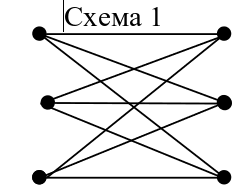
\includegraphics[scale=0.5]{pics/graph_1.png}
       \end{center}
    \end{minipage}

    \vspace{1em}
    \begin{center}
        \textbf{Расчеты}
    \end{center}

    \begin{minipage}{.45\linewidth}
        \begin{tikzpicture}[node distance={2cm}, main/.style = {draw, circle}] 
            \node[main] (1) {$M1$}; 
            \node[main] (2) [below of=1] {$M2$}; 
            \node[main] (3) [below of=2] {$M3$}; 
            \node[main] (4) [right of=1, xshift=2cm] {$E1$}; 
            \node[main] (5) [right of=2, xshift=2cm] {$E2$}; 
            \node[main] (6) [right of=3, xshift=2cm] {$E3$}; 
            \draw[draw=green, very thick] (1) -- (4);
            \draw[draw=red, very thick] (1) -- (5);
            \draw[draw=blue, very thick] (1) -- (6);
            \draw[draw=blue, very thick] (2) -- (4);
            \draw[draw=green, very thick] (2) -- (5);
            \draw[draw=red, very thick] (2) -- (6);
            \draw[draw=red, very thick] (3) -- (4);
            \draw[draw=blue, very thick] (3) -- (5);
            \draw[draw=green, very thick] (3) -- (6);
        \end{tikzpicture}

        \begin{tikzpicture}
            \draw[draw=green, very thick] (-2,1) -- (3,1) node [pos=0.5, above] {$K1$};
            \draw[draw=red, very thick] (-2,0) -- (3,0) node [pos=0.5, above] {$K2$};
            \draw[draw=blue, very thick] (-2,-1) -- (3,-1) node [pos=0.5, above] {$K3$};
        \end{tikzpicture}

    \end{minipage}
    \begin{minipage}{.45\linewidth}
    \underline{Расчет сумм вероятностей ключей:}\\
    \noindent$P(E_1|M_1)=\sum_s P(K)_s = \frac{1}{3}$\\
    $P(E_1|M_2)=\sum_s P(K)_s = \frac{1}{3}$\\
    $P(E_1|M_3)=\sum_s P(K)_s = \frac{1}{3}$\\
    $P(E_2|M_1)=\sum_s P(K)_s = \frac{1}{3}$\\
    $P(E_2|M_2)=\sum_s P(K)_s = \frac{1}{3}$\\
    $P(E_2|M_3)=\sum_s P(K)_s = \frac{1}{3}$\\
    $P(E_3|M_1)=\sum_s P(K)_s = \frac{1}{3}$\\
    $P(E_3|M_2)=\sum_s P(K)_s = \frac{1}{3}$\\
    $P(E_3|M_3)=\sum_s P(K)_s = \frac{1}{3}$\\
    \end{minipage}\\
    \underline{Расчет вероятностей криптограмм:}\\
    \noindent$P(E_1)=P(M_1)P(E_1|M_1)+P(M_2)P(E_1|M_2)+P(M_3)P(E_1|M_3)=0.4\cdot\frac{1}{3}+0.5\cdot\frac{1}{3}+0.1\cdot\frac{1}{3}=\frac{1}{3}$\\
    $P(E_2)=P(M_1)P(E_2|M_1)+P(M_2)P(E_2|M_2)+P(M_3)P(E_2|M_3)=0.4\cdot\frac{1}{3}+0.5\cdot\frac{1}{3}+0.1\cdot\frac{1}{3}=\frac{1}{3}$\\
    $P(E_3)=P(M_1)P(E_3|M_1)+P(M_2)P(E_3|M_2)+P(M_3)P(E_3|M_3)=0.4\cdot\frac{1}{3}+0.5\cdot\frac{1}{3}+0.1\cdot\frac{1}{3}=\frac{1}{3}$\\

    \underline{Расчет апостериорных вероятностей всех сообщений:}\\
    \noindent$P(M_1|E_1)=\frac{P(E_1|M_1)P(M_1)}{P(E_1)}=\frac{\frac{1}{3}\cdot0.4}{\frac{1}{3}}=0.4$\\
    $P(M_1|E_2)=\frac{P(E_2|M_1)P(M_1)}{P(E_2)}=\frac{\frac{1}{3}\cdot0.4}{\frac{1}{3}}=0.4$\\
    $P(M_1|E_3)=\frac{P(E_3|M_1)P(M_1)}{P(E_3)}=\frac{\frac{1}{3}\cdot0.4}{\frac{1}{3}}=0.4$\\
    $P(M_2|E_1)=\frac{P(E_1|M_2)P(M_2)}{P(E_1)}=\frac{\frac{1}{3}\cdot0.5}{\frac{1}{3}}=0.5$\\
    $P(M_2|E_2)=\frac{P(E_2|M_2)P(M_2)}{P(E_2)}=\frac{\frac{1}{3}\cdot0.5}{\frac{1}{3}}=0.5$\\
    $P(M_2|E_3)=\frac{P(E_3|M_2)P(M_2)}{P(E_3)}=\frac{\frac{1}{3}\cdot0.5}{\frac{1}{3}}=0.5$\\
    $P(M_3|E_1)=\frac{P(E_1|M_3)P(M_3)}{P(E_1)}=\frac{\frac{1}{3}\cdot0.1}{\frac{1}{3}}=0.1$\\
    $P(M_3|E_2)=\frac{P(E_2|M_3)P(M_3)}{P(E_2)}=\frac{\frac{1}{3}\cdot0.1}{\frac{1}{3}}=0.1$\\
    $P(M_3|E_3)=\frac{P(E_3|M_3)P(M_3)}{P(E_3)}=\frac{\frac{1}{3}\cdot0.1}{\frac{1}{3}}=0.1$\\
    \textbf{Выводы}

    Т.к. $P(M_1|E_j)=P(M_1)$, $P(M_2|E_j)=P(M_2)$, $P(M_3|E_j)=P(M_3)$, то система шифрования 
    является безусловно стойкой из условия АССШ $P(M|E) = P(M)$.
\end{document}